\documentclass[tikz]{standalone}
\usepackage[utf8]{inputenc}
\usetikzlibrary{calc,intersections}

\begin{document}

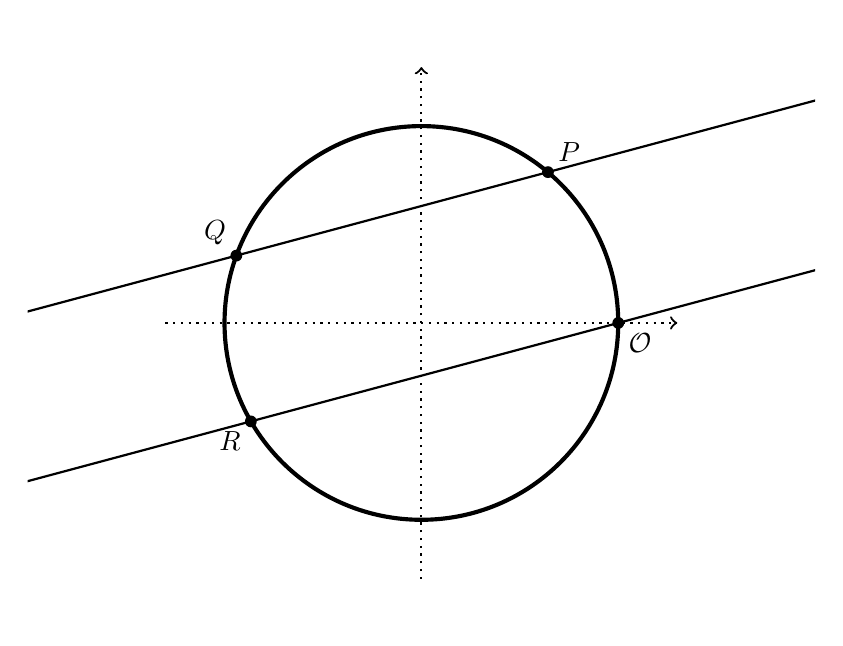
\begin{tikzpicture}[thick,scale=2.5]
\def\ptsize{.03}
\newcount\Pangle
\newcount\Qangle
\newcount\Rangle
\Pangle=50
\Qangle=160
\Rangle=\Pangle
\advance\Rangle by \Qangle
\draw[->,dotted] (-1.3, 0) -- (1.3,0);
\draw[->,dotted] (0,-1.3) -- (0,1.3);
\clip (-2,-1.5) rectangle (2,1.5);
\path[draw,name path=circ,line width=1.5pt] (0,0) circle (1);
\coordinate[label=below right:$\mathcal{O}$] (inf) at (1,0);
\coordinate[label=above right:$P$] (P) at (\number\Pangle:1);
\coordinate[label=above left:$Q$] (Q) at (\number\Qangle:1);
\coordinate[label=below left:$R$] (R) at (\number\Rangle:1);
\fill (inf) circle (\ptsize);
\fill (P) circle (\ptsize);
\fill (Q) circle (\ptsize);
\fill (R) circle (\ptsize);
\draw[shorten >=-10cm,shorten <=-10cm] (P) -- (Q);
\path[name path=lineOR,draw,shorten >=-10cm,shorten <=-10cm] (inf) -- +($(P)-(Q)$);
\end{tikzpicture}

\end{document}